\hypertarget{cv:gestionarPantallas}{\section{Gestionar Pantallas}} \label{sec:GestionarPantallas}

	Esta funcionalidad le permitirá las acciones necesarias para controlar las pantallas asi como sus acciones y visualizarlos en una tabla en el proyecto sobre el que se está operando y solicitar el registro de uno nuevo.

		\subsection{Procedimiento}

			%Pasos de procedimiento
			\begin{enumerate}
				
			\item Ingrese a un proyecto existente desde la pantalla \ref{fig:GestionarProyectosColaborador}.
	
			\item Oprima el botón \IUPantallas{} de algún registro existente de la pantalla \ref{fig:GestionarModulos} ''Gestionar Módulos''.
	
			\item Se mostrará la pantalla \ref{fig:GestionarPantallas} ''Gestionar Pantallas''.

			%Pantalla
			\begin{figure}[h!]
				\begin{center}
					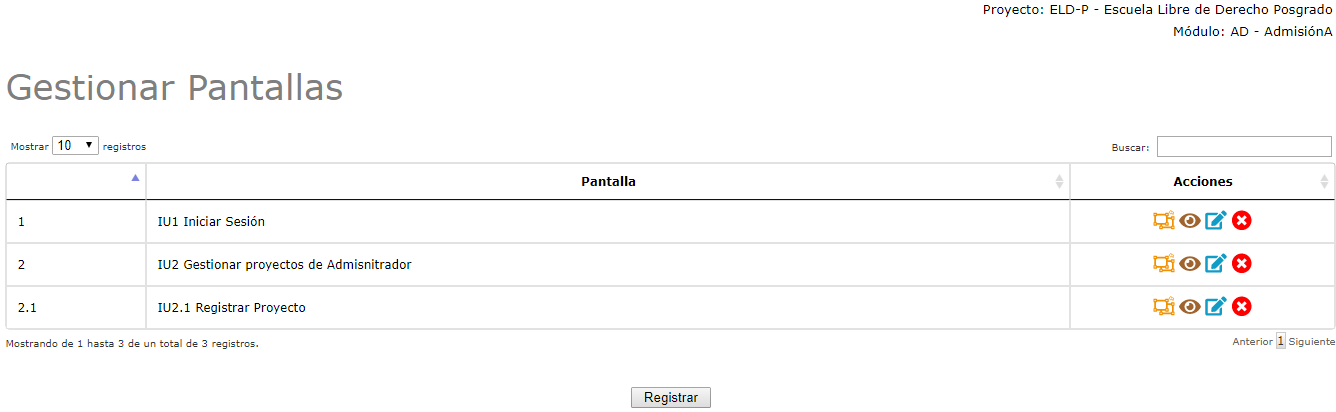
\includegraphics[scale=0.5]{roles/lider/pantallas/pantallas/IU11gestionarPantallas}
					\caption{Gestionar Pantallas}
					\label{fig:GestionarPantallas}
				\end{center}
			\end{figure}
		
				\item Seleccione la operación que desea realizar:
			
			Para (\hyperlink{cv:registrarPantalla}{Registrar}) dé clic en el botón \IURegistrar.
			
			Para (\hyperlink{cv:modificarPantalla}{Modificar}) dé clic en el icono \IUEditar{} de alguna pantalla ya registrada.
			
			Para (\hyperlink{cv:eliminarPantalla}{Eliminar}) dé clic en el icono \IUBotonEliminar{} de alguna pantalla ya registrada.
			
			Para (\hyperlink{cv:consultarPantalla}{Consultar}) dé clic en el icono \IUConsultar{} de alguna pantalla ya registrada.
			
			Para (\hyperlink{cv:gestionarAcciones}{Gestionar los atributos}) dé clic en el icono \IUAcciones{} de alguna pantalla ya registrada.
			\end{enumerate}